\documentclass[12pt,a4paper]{article}
% Estilo compartido para informes. Compilar con LuaLaTeX desde tp1/.
\usepackage[spanish,es-nodecimaldot]{babel}
\usepackage{fontspec}
\setmainfont{Montserrat-Medium.ttf}[
  Path=../assets/fonts/,
  BoldFont=Montserrat-Bold.ttf,
  ItalicFont=Montserrat-MediumItalic.ttf]
\usepackage[a4paper,margin=2.5cm,headheight=16pt]{geometry}
\usepackage{xcolor,graphicx,booktabs,tabularx}
\usepackage{float}
\usepackage{titlesec,fancyhdr,enumitem,caption}
\usepackage{ragged2e}
\usepackage{hyperref}
\definecolor{verde}{HTML}{1D4036}
\definecolor{bronce}{HTML}{D38129}
\definecolor{rosa}{HTML}{D88E77}
\definecolor{calido}{HTML}{EFE4D8}
\definecolor{grafito}{HTML}{1D1D1D}
\hypersetup{colorlinks=true,linkcolor=verde,urlcolor=verde,
  pdftitle={TP1 - Instalación de máquinas virtuales},pdfsubject={Cyberseguridad}}
\AtBeginDocument{\color{grafito}\RaggedRight\fontsize{12}{14.4}\selectfont}
\setlength{\parindent}{0pt}
\setlength{\parskip}{7pt}
\setlist[itemize]{leftmargin=*,itemsep=7pt,topsep=4pt}
\setlist[enumerate]{leftmargin=*,itemsep=6pt}
\titleformat{\section}{\color{verde}\bfseries\fontsize{18}{21.6}\selectfont}{\thesection}{0.65em}{}
\titleformat{\subsection}{\color{verde}\bfseries\large}{\thesubsection}{0.65em}{}
\titleformat{\subsubsection}{\color{verde}\bfseries}{\thesubsubsection}{0.65em}{}
\titlespacing*{\section}{0pt}{16pt}{8pt}
\titlespacing*{\subsection}{0pt}{12pt}{5pt}
\titlespacing*{\subsubsection}{0pt}{10pt}{4pt}
\setcounter{tocdepth}{2}
\pagestyle{fancy}
\fancyhf{}
\fancyhead[L]{\small\color{verde}FCEFyN | UNC}
\fancyhead[R]{\small\color{verde}\materia\ · TP \numeroTP}
\fancyfoot[L]{\scriptsize Informe de laboratorio}
\fancyfoot[R]{\small\thepage}
\renewcommand{\headrulewidth}{0.4pt}
\captionsetup{font=small,labelfont=bf,justification=raggedright,singlelinecheck=false,hypcap=false}
\newcommand{\pendiente}[1]{\par{\small\color{verde}\textbf{Por completar.} #1\par}}
% Si falta una captura se muestra un espacio reservado; no impide compilar.
\newcommand{\captura}[2]{%
  \par\smallskip\begingroup\centering
  \IfFileExists{figuras/#1}{%
    \includegraphics[width=\linewidth,height=5cm,keepaspectratio]{figuras/#1}%
  }{%
    \setlength{\fboxsep}{10pt}%
    \fcolorbox{bronce}{calido}{\parbox[c][1.25cm][c]{\dimexpr\linewidth-2\fboxsep-2\fboxrule\relax}{%
      \centering\small Captura pendiente\par\texttt{\detokenize{#1}}}}%
  }%
  \captionof{figure}{#2}\par\endgroup\smallskip
}

\usepackage{xurl}

\newcommand{\materia}{Cyberseguridad}
\newcommand{\numeroTP}{12}
\newcommand{\tituloTP}{Cifrado con OpenSSL}
\newcommand{\estudiante}{Brigido Tomas Andres}
\newcommand{\legajo}{38481096}
\newcommand{\carrera}{ICOMP}
\newcommand{\docente}{Javier A. Jorge}


% Metadatos específicos del TP12 y capturas en img/.
\hypersetup{pdftitle={TP12 - Cifrado con OpenSSL}}
\renewcommand{\captura}[2]{%
  \begin{figure}[H]
    \centering
    \IfFileExists{img/#1}{%
      \includegraphics[width=0.85\linewidth,height=5cm,keepaspectratio]{img/#1}%
    }{%
      \setlength{\fboxsep}{10pt}%
      \fcolorbox{bronce}{calido}{\parbox[c][1.1cm][c]{0.85\linewidth}{%
        \centering\small Captura pendiente\par\texttt{\detokenize{#1}}}}%
    }%
    \caption{#2}
  \end{figure}
}

\usepackage{caption}
\captionsetup{justification=centering}
\begin{document}
\hypersetup{pageanchor=false}
\begin{titlepage}
  
\includegraphics[width=8cm]{../assets/logo-fcefyn-2026.png}
  \vspace{1cm}

  {\color{verde}\small UNIVERSIDAD NACIONAL DE CÓRDOBA\par}
  \vspace{2.1cm}
  {\color{bronce}\bfseries\large TRABAJO PRÁCTICO \numeroTP\par}
  \vspace{0.45cm}
  {\color{verde}\bfseries\fontsize{32}{38.4}\selectfont Cifrado con\\OpenSSL\par}
  \vspace{0.3cm}
{\small Criptografía simétrica, asimétrica e híbrida\par}
\vspace{0.35cm}
  {\large \materia\par}
  \vspace{0.8cm}
  {\color{bronce}\rule{2.7cm}{2pt}\par}
  \vfill
  \renewcommand{\arraystretch}{1.45}
  \begin{tabular}{@{}p{3.2cm}p{10cm}@{}}
    Estudiante & \estudiante \\
    Legajo & \legajo \\
    Carrera & \carrera \\
    Docente & \docente \\
  \end{tabular}
  \vfill
  {\small Córdoba, Argentina\par}
\end{titlepage}
\hypersetup{pageanchor=true}

\tableofcontents
\vspace{1cm}
\newpage

\section{Introducción y objetivos}
Esta práctica propone cifrar y descifrar mensajes y archivos con OpenSSL, utilizando criptografía simétrica, asimétrica e híbrida. Se documentarán los comandos empleados y se comprobará la recuperación de los datos originales.


\section{Criptografía simétrica}
\subsection{Cifrado de un archivo de texto}

\begin{figure}[H]
    \centering
    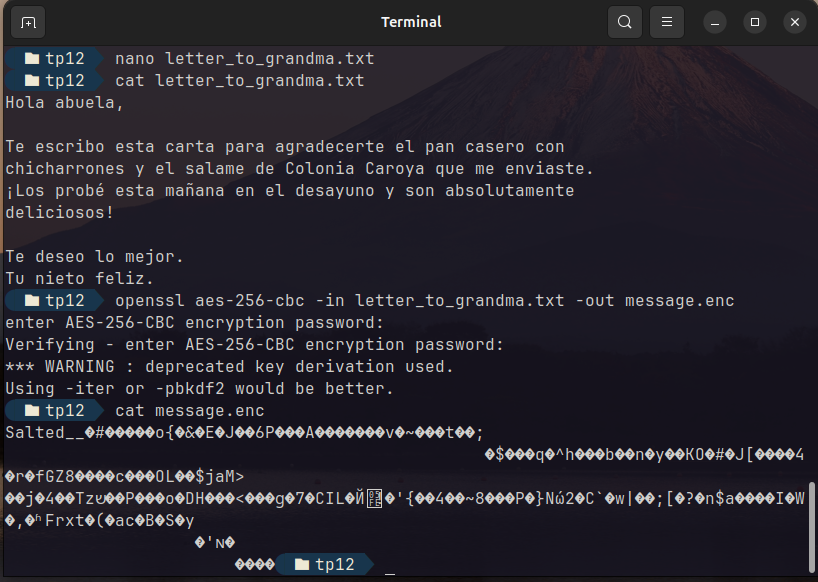
\includegraphics[width=0.9\textwidth]{img/cartaencriptada.png}
    \caption{Cifrado simétrico del mensaje.}
    \label{fig:una-imagen}
\end{figure}

\begin{figure}[H]
    \centering
    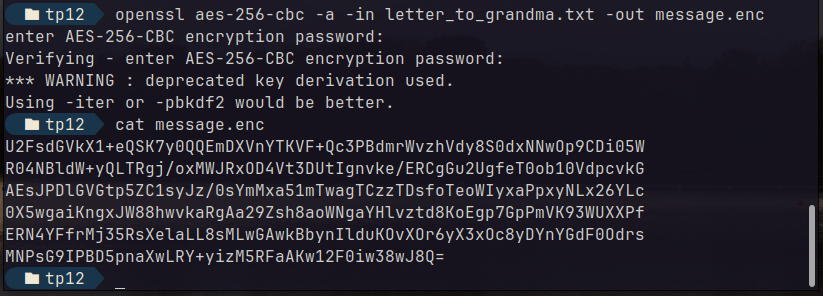
\includegraphics[width=0.9\textwidth]{img/encriptacionconbandera.png}
    \caption{Cifrado simétrico con la bandera -a.}
    \label{fig:una-imagen}
\end{figure}
\par\textbf{¿Puede pensar en algún beneficio de tener message.enc codificado como Base64?}

Base64 representa los datos binarios del archivo cifrado mediante caracteres de texto, facilitando su envío por correo o su copia sin problemas con caracteres no imprimibles. No añade seguridad, es una codificación, no un cifrado.

\subsection{Descifrado y verificación}
\begin{figure}[H]
    \centering
    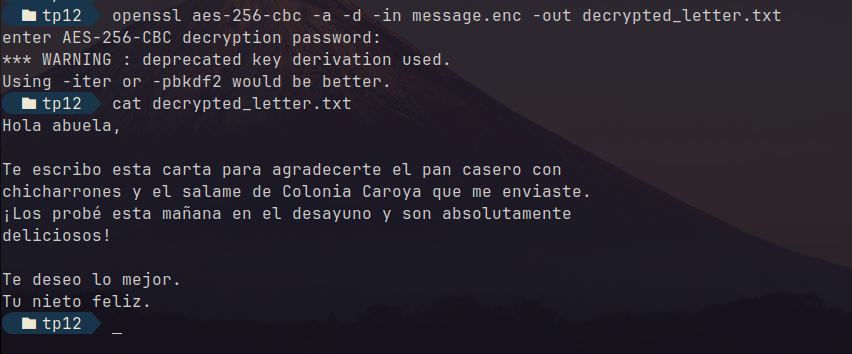
\includegraphics[width=0.9\textwidth]{img/decripted.png}
    \caption{Archivo recuperado mediante descifrado simétrico.}
    \label{fig:una-imagen}
\end{figure}
\par\textbf{Observe que el comando que se utilizó para descifrar también contiene una opción -a. ¿Puede explicarlo?}

La opción \texttt{-a} indica que OpenSSL debe decodificar el archivo de Base64 antes de descifrarlo, porque se utilizó esa codificación al guardar el mensaje cifrado.

\section{Criptografía asimétrica}
\subsection{Generación y extracción de claves}
Los dos pares de claves se generaron con las contraseñas privadas \texttt{contraseñaalice} y \texttt{contraseñabob}.  

\begin{figure}[H]
    \centering
    \begin{minipage}{0.48\textwidth}
        \centering
        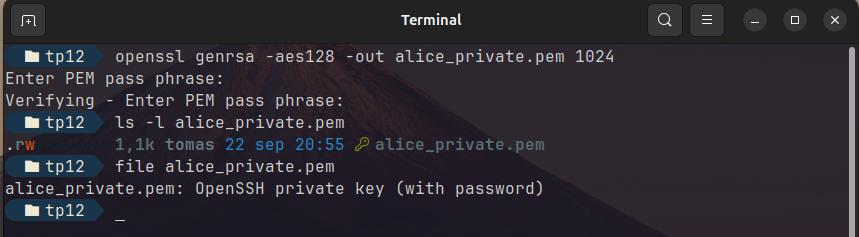
\includegraphics[width=\linewidth]{img/aliceparclave.png}
        \caption{Generación de la clave privada de Alice.}
        \label{fig:dos-primera}
    \end{minipage}
    \hfill
    \begin{minipage}{0.48\textwidth}
        \centering
        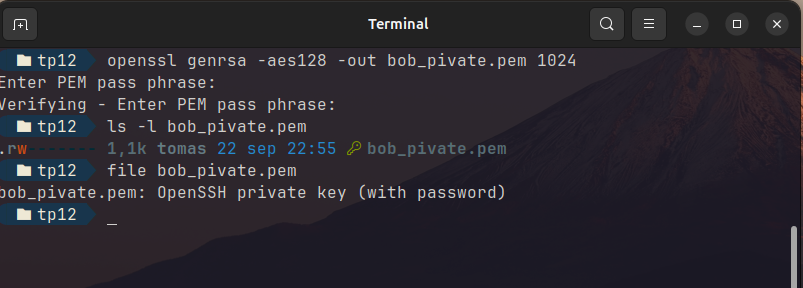
\includegraphics[width=\linewidth]{img/bobparclave.png}
        \caption{Generación de la clave privada de Bob.}
        \label{fig:dos-segunda}
    \end{minipage}
\end{figure}

Podemos ver la clave privada de Alice en las siguentes capturas. 

\begin{figure}[H]
    \centering
    \begin{minipage}[t]{0.48\textwidth}
        \vspace{0pt}
        \centering
        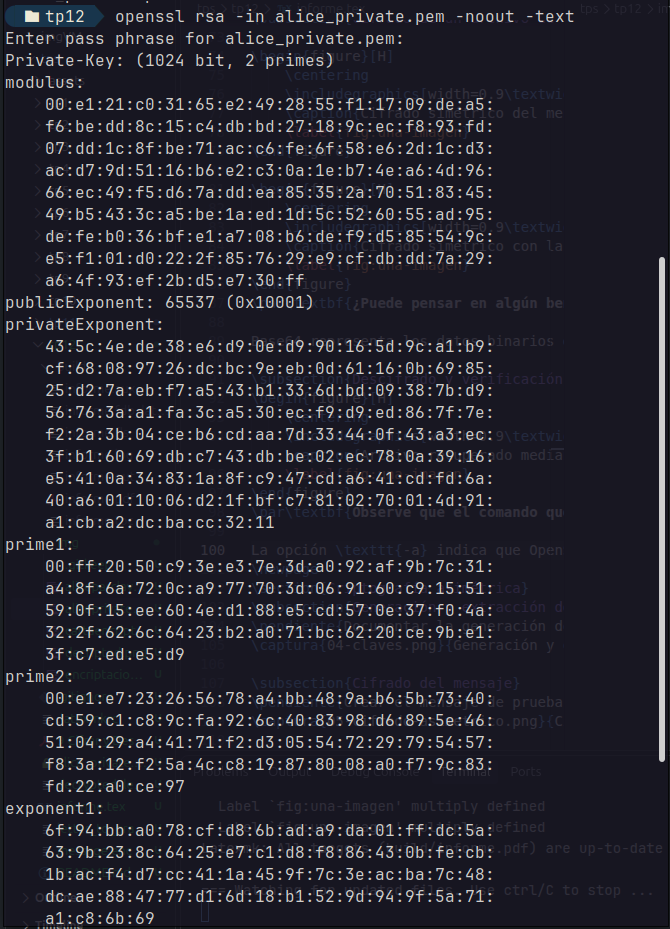
\includegraphics[width=\linewidth]{img/alice1.png}
        \caption{Clave privada de Alice.}
        \label{fig:larga}
    \end{minipage}
    \hfill
    \begin{minipage}[t]{0.48\textwidth}
        \vspace{0pt}
        \centering
        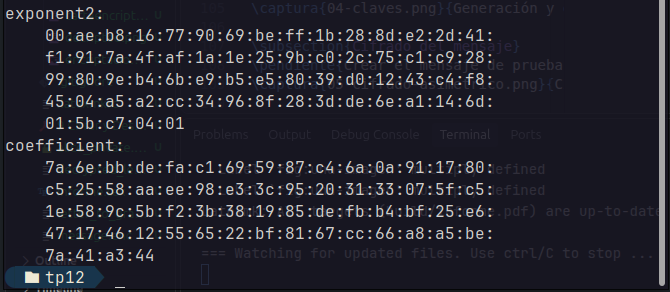
\includegraphics[width=\linewidth]{img/alice2.png}
        \caption{Clave privada de Alice.}
        \label{fig:corta1}

        \bigskip

        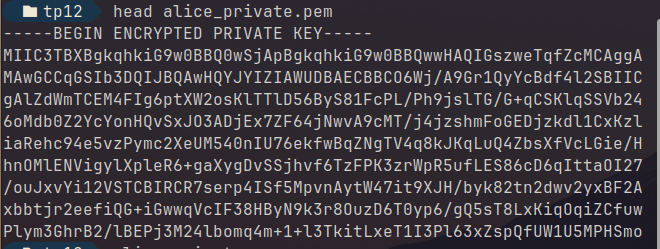
\includegraphics[width=\linewidth]{img/alice0.png}
        \caption{Clave privada de Alice encriptada.}
        \label{fig:corta2}
    \end{minipage}
\end{figure}

Podemos extraer la clave pública de Alice con el siguiente comando:
\begin{figure}[H]
    \centering
    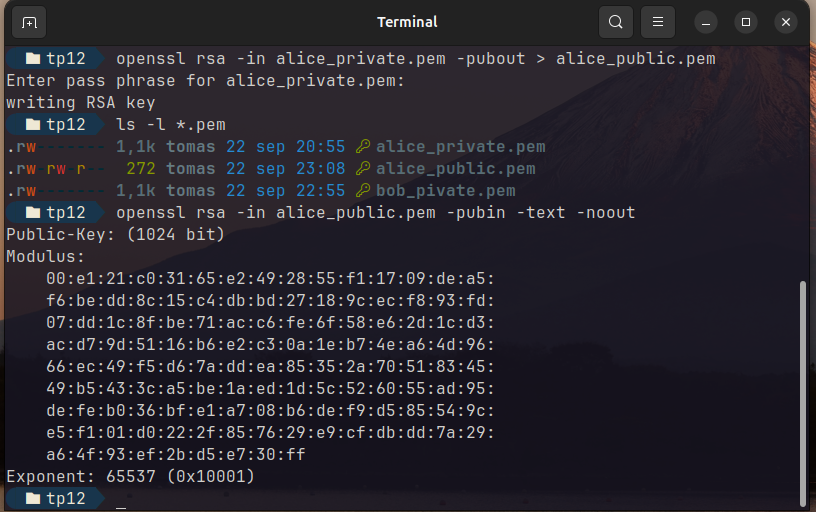
\includegraphics[width=0.9\textwidth]{img/aliceclavepublica.png}
    \caption{Clave pública de Alice.}
    \label{fig:una-imagen}
\end{figure}

Terminamos generando los pares claves publico y privado de Bob y de Alice. 
\begin{figure}[H]
    \centering
    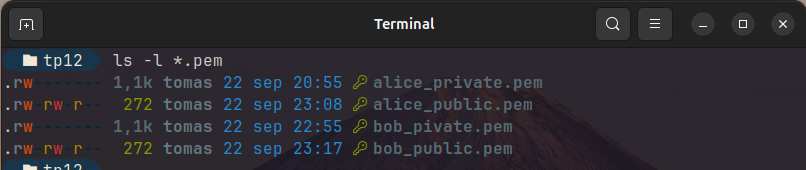
\includegraphics[width=0.9\textwidth]{img/parclaves.png}
    \caption{Pares de claves.}
    \label{fig:una-imagen}
\end{figure}

\subsection{Cifrado del mensaje}

Con la clave pública de Bob, Alice puede cifrar un mensaje para él.
\begin{figure}[H]
    \centering
    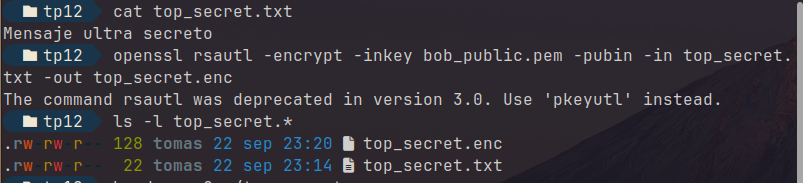
\includegraphics[width=0.9\textwidth]{img/msjabobencript.png}
    \caption{Mensaje cifrado para Bob.}
    \label{fig:una-imagen}
\end{figure}

\begin{figure}[H]
    \centering
    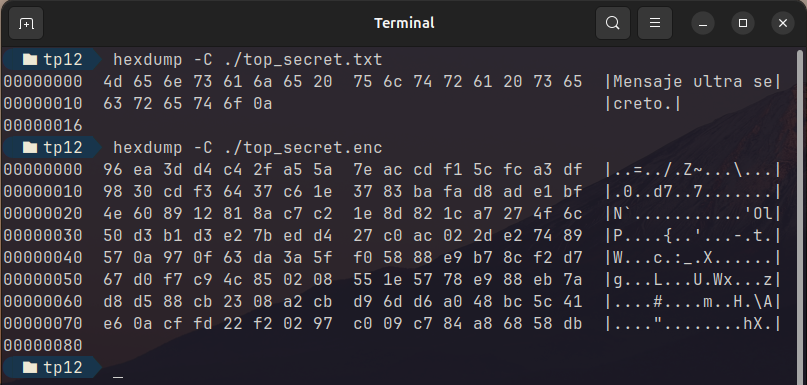
\includegraphics[width=0.9\textwidth]{img/hexdump.png}
    \caption{Visualización en hexadecimal del mensaje cifrado.}
    \label{fig:una-imagen}
\end{figure}

\subsection{Descifrado e intercambio inverso}

Luego con su clave privada, Bob puede descifrar el mensaje que Alice le envió.

\begin{figure}[H]
    \centering
    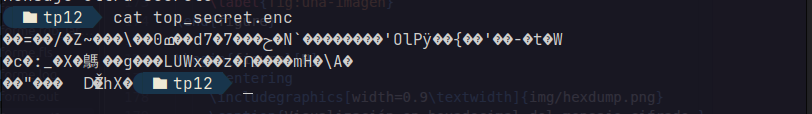
\includegraphics[width=0.9\textwidth]{img/msjabobencriptado.png}
    \caption{Mensaje cifrado recibido por Bob.}
    \label{fig:una-imagen}
\end{figure}

\begin{figure}[H]
    \centering
    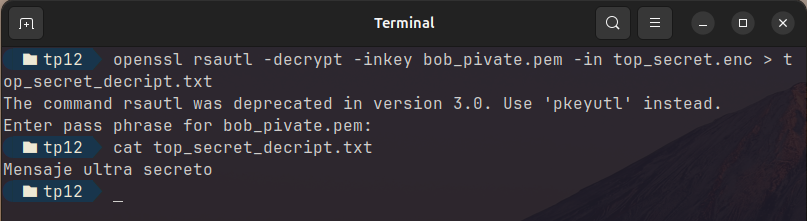
\includegraphics[width=0.9\textwidth]{img/msjabob.png}
    \caption{Mensaje descifrado por Bob.}
    \label{fig:una-imagen}
\end{figure}

\newpage
\section{Referencias}
Cisco Networking Academy. \textit{Cifrar y descifrar datos y archivos con OpenSSL}. Consigna proporcionada para la actividad.
\end{document}
